\documentclass[10pt]{beamer}
\usepackage[utf8]{inputenc}
\usepackage{hyperref}
\usepackage[scaled]{helvet}
\usepackage[T1]{fontenc}
\usetheme{Berkeley}
\beamertemplatenavigationsymbolsempty
\setbeamertemplate{headline}{}
\setbeamersize{sidebar width left=1.5cm}
\setbeamerfont{section in sidebar}{size=\fontsize{6}{6}\selectfont}
\setbeamerfont{title in sidebar}{size=\fontsize{6}{6}\selectfont}
\title{Data Collection and Import}
\date{}

\begin{document}
\maketitle

\section{Topics}
\begin{frame}
\leftskip1em\textbf{Learn}
	\begin{itemize}
		\item to fill in a Start Tracing Backward template
    \item to import templates
    \item to load data into the KNIME workflow
	\end{itemize}
\end{frame}

\section{1}
\begin{frame}
	\begin{center}
		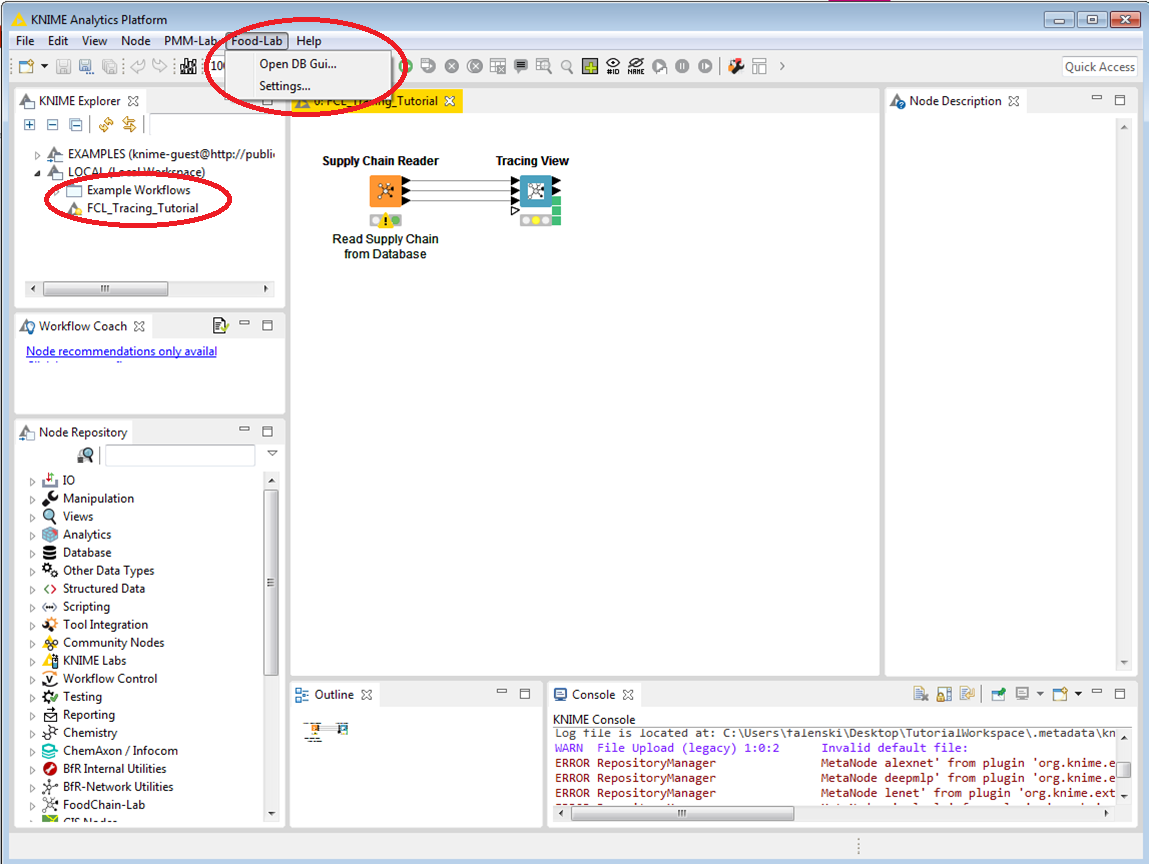
\includegraphics[height=0.6\textheight]{1.png}
	\end{center}
	\begin{itemize}
		\item Open the workflow \href{https://github.com/SiLeBAT/BfROpenLabResources/raw/master/GitHubPages/workflows/FCL_Tracing_Tutorial.knwf}{``FCL\_Tracing\_Tutorial.knwf''} from the tracing tutorial.
    \item Open the database
	\end{itemize}
\end{frame}

\section{2}
\begin{frame}
	\begin{center}
			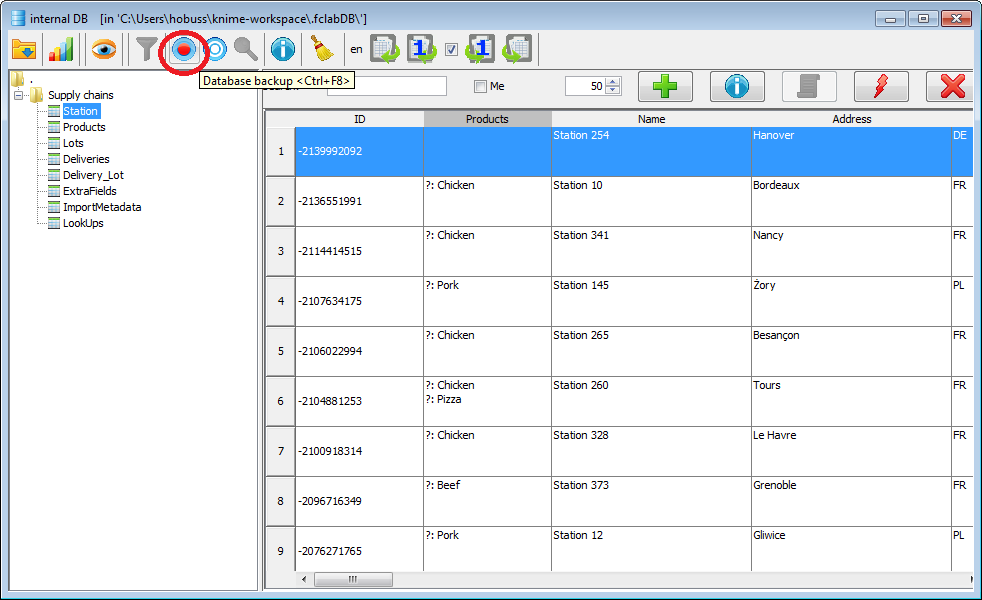
\includegraphics[height=0.6\textheight]{2.png}
	\end{center}
	\begin{itemize}
		\item We need an empty database. Before we reset the database, you can produce a backup: Click the button for backup. A window opens. Choose a folder in which you would like to save your data and click "save".
	\end{itemize}
\end{frame}

\section{3}
\begin{frame}
	\begin{center}
			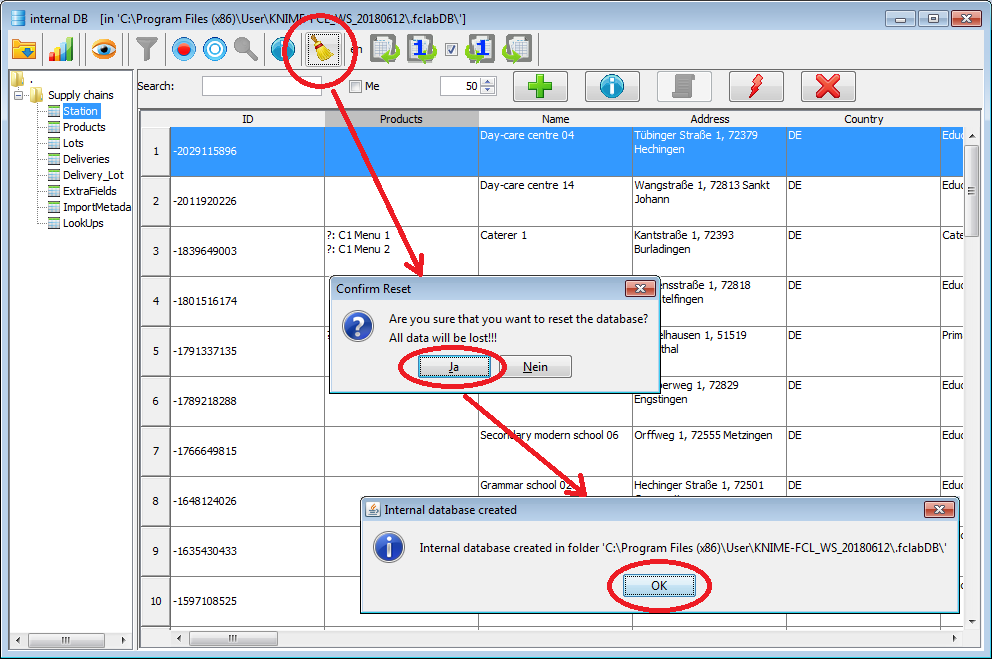
\includegraphics[height=0.6\textheight]{3.png}
	\end{center}
	\begin{itemize}
		\item Use the broom to sweep your database clean.
		\item Confirm that you would like to reset the database with „Ja“. The database closes and a new empty database is created.
		\item Click "OK".
	\end{itemize}
\end{frame}

\section{4}
\begin{frame}
\leftskip1em{In Excel:}
	\begin{itemize}
		\item Open the empty template \href{https://foodrisklabs.bfr.bund.de/wp-content/uploads/2015/11/FCL_Backtrace_Start_tob_en.xlsx}{``FCL\_Backtrace\_Start\_tob\_en.xlsx''} and fill in the data from the delivery papers (see \href{https://github.com/SiLeBAT/BfROpenLabResources/raw/master/GitHubPages/documents/foodchainlab_datacollectimport/Dry-Stuff-Inc_START-tracing.docx}{``Dry-Stuff-Inc\_START-tracing.docx''})
		\item Save the excel template with a different name.
	\end{itemize}
\end{frame}

\section{5a}
\begin{frame}
\leftskip1em{In KNIME:}
	\begin{center}
			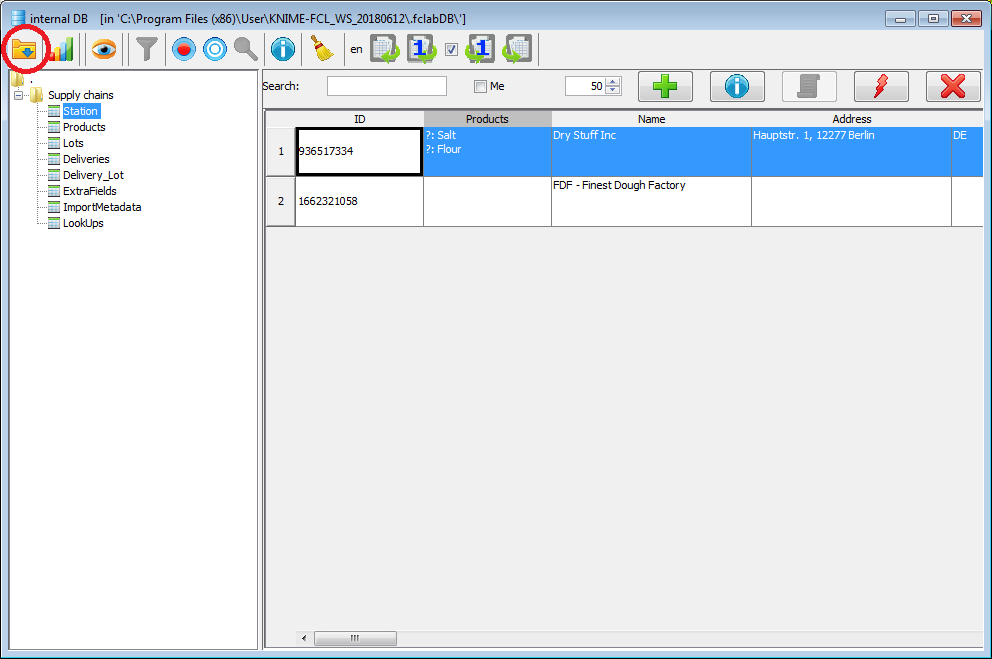
\includegraphics[height=0.6\textheight]{5a.png}
	\end{center}
	\begin{itemize}
		\item Import your file into the database (see import button in the red circle).
		\item Also import \href{https://github.com/SiLeBAT/BfROpenLabResources/raw/master/GitHubPages/documents/foodchainlab_datacollectimport/All_In_One_Template_Cake-Scenario.xlsx}{``All\_In\_One\_Template\_Cake-Scenario.xlsx''}).
	\end{itemize}
\end{frame}

\section{5b}
\begin{frame}
	\begin{center}
			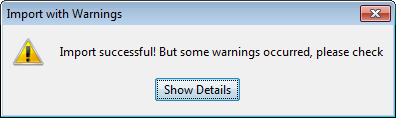
\includegraphics[scale=0.5]{5b.png}
	\end{center}
	\begin{itemize}
		\item A warning appears informing you that there is a difference in the weight of incoming goods to that of outgoing goods for a specific lot. For this tutorial it does not matter that we do not know anything about the remaining 499.1 kg.
	\end{itemize}
	\begin{center}
			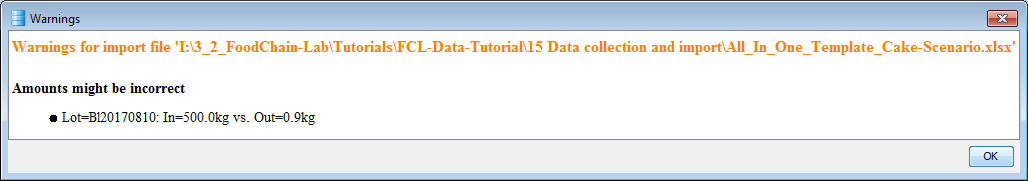
\includegraphics[scale=0.375]{5c.png}
	\end{center}
	\begin{itemize}
		\item Close the window by clicking ``OK''.
	\end{itemize}
\end{frame}

\section{6}
\begin{frame}
	\begin{center}
			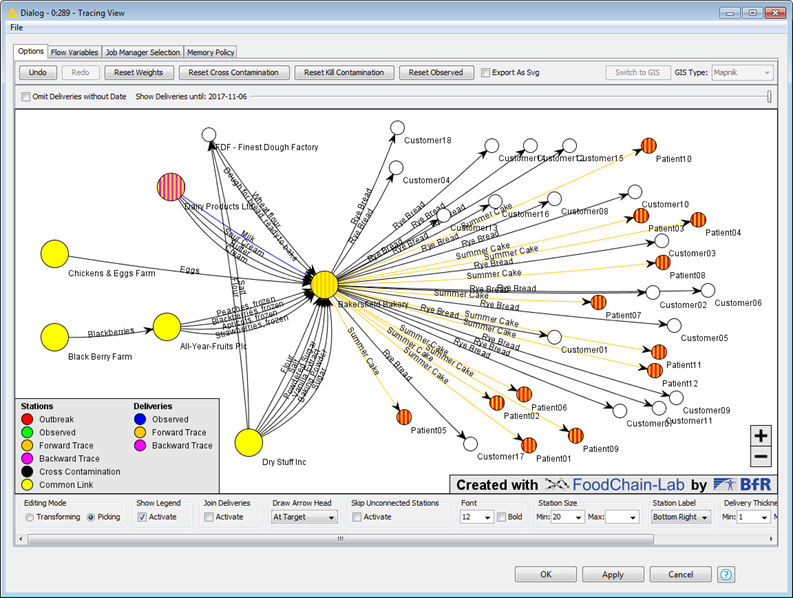
\includegraphics[height=0.6\textheight]{6.png}
	\end{center}
	\begin{itemize}
		\item Close the database, reset the Supply Chain Reader and double click the Tracing View (the Supply Chain Reader is then executed automatically).
		\item Again: Have a look at the Tracing View. The network should have the same structure as the one above (perhaps with different colours).
	\end{itemize}
\end{frame}

\end{document}
